\documentclass[10pt, a4paper]{article}

% \usepackage[mathdisplays=normal]{savetrees}

% Core packages for better typography
\usepackage[utf8]{inputenc}
\usepackage[T1]{fontenc}
\usepackage{lmodern}
% \usepackage{newtxtext,newtxmath}
\usepackage{latexsym,amsfonts,amssymb,amsthm,amsmath}
\usepackage{mathtools}
\usepackage{textcomp}
\usepackage{microtype}
\usepackage{setspace}
\usepackage{siunitx}
\DeclareSIUnit{\um}{\ensuremath{\mu}\mathrm{m}}
% \onehalfspacing

% Math packages with better formatting

% Graphics and figures
\usepackage{tikz}
\usetikzlibrary{angles,quotes}
\usepackage{pgfplots}
\pgfplotsset{compat=newest}
\usepackage{graphicx}
\graphicspath{{../data/}}

% Better table formatting
\usepackage{booktabs}
\usepackage{array}
\usepackage{multirow}

% Force figures to stay in their sections
\usepackage[section]{placeins}
\makeatletter
\AtBeginDocument{%
  \expandafter\renewcommand\expandafter\subsection\expandafter{%
    \expandafter\@fb@secFB\subsection
  }%
}
\makeatother

% Code listing formatting
\usepackage{listings}
\usepackage{xcolor}
\definecolor{codegreen}{rgb}{0,0.6,0}
\definecolor{codegray}{rgb}{0.5,0.5,0.5}
\definecolor{codepurple}{rgb}{0.58,0,0.82}
\definecolor{backcolour}{rgb}{0.95,0.95,0.92}
\lstdefinestyle{mystyle}{
  backgroundcolor=\color{backcolour},   
  commentstyle=\color{codegreen},
  keywordstyle=\color{blue},
  numberstyle=\tiny\color{codegray},
  stringstyle=\color{codepurple},
  basicstyle=\ttfamily\footnotesize,
  breakatwhitespace=false,         
  breaklines=true,                 
  captionpos=b,                    
  keepspaces=true,                 
  showspaces=false,                
  showstringspaces=false,
  showtabs=false,                  
  tabsize=2
}
\lstset{style=mystyle}

% References and hyperlinks
\usepackage{pdfpages}
\usepackage[colorlinks=true, linkcolor=blue, citecolor=blue]{hyperref}
\usepackage{caption}
\usepackage{subcaption}
\usepackage{csquotes}
\usepackage[notes, backend=bibtex]{biblatex-chicago}
\addbibresource{refs.bib}



% Custom theorem environments
\newtheorem{theorem}{Theorem}[section]
\newtheorem{lemma}[theorem]{Lemma}
\newtheorem{proposition}[theorem]{Proposition}
\newtheorem{corollary}[theorem]{Corollary}
\newtheorem{definition}{Definition}[section]
\newtheorem{example}{Example}[section]

\title{\Large \bfseries SB4: Integrated Photonics\\[0.5em] \large Final Report}
\author{Lucas Ng\thanks{ln373@cam.ac.uk}}
\date{13th June 2025}

\begin{document}
\maketitle

\section{Introduction}

In the first interim report, we performed modal analysis on a symmetric planar waveguide
of several core and cladding materials, with further investigation into the effects of waveguide geometry and modal excitation wavelength on the modal properties,
including the effective index, group index, birefringence, and dispersion characteristics.

The second interim report recognised that waveguides do not exist in isolation,
and presented the coupled mode theory as a framework for understanding the power transfer across coupled waveguides,
with a derivation via considering the coupled mode propagation matrix,
\[
\mathbf{M} = \begin{pmatrix}
\beta & \kappa \\
\kappa & \beta
\end{pmatrix},
\]
to be the infinitessimal generator matrix that generates the modal evolution transition matrix as 
a one-parameter subgroup of the Lie group \(GL(2, \mathbb{C})\)
via the exponential map \(-jzM\mapsto e^{-jzM}\) (where \(z\) is the propagation distance along the waveguide)
that acts on an element of the Lie algebra \(\mathfrak{gl}(2, \mathbb{C})\).
This formalism demonstrated how the intrinsic structure of \(M\) gives rise to the modal properties of the coupled waveguide:
the symmetry of the matrix \(M\) corresponds to reciprocal coupling,
while real-valued \(\beta\) and \(\kappa\) encodes the conservation of power in the coupled waveguide,
since in this instance, \(-jzM\) is Hermitian, and thus the image of the exponential map is unitary.

Likewise, this current, final report, ascends to the next level of abstraction,
\textit{\'a la mise en abyme},
considering the whole structure of a S-bend directional coupler in its entirety.
At this level, the previous theoretical frameworks serve purely as approximation,
and we must account for bending losses, asymmetric couplers, and other practical and interesting considerations.
This being analytically intractable, Lumerical's FDTD software\autocite{lumerical_fdtd} was utilised to simulate the directional coupler.

\section{Simulation setup}

The geometry of our directional coupler is the traditional doubly-symmetric S-bend design,
with a parallel coupling length connected in each waveguide to its input and output ports by S-bends.
Each port is extended by a straight waveguide which extends through to \SI{1}{\um} outside the FDTD simulation region,
which is otherwise internally padded on all sides by \SI{2.5}{\um} of perfectly matched layer (PML) boundary conditions.
The input port of the upper waveguide is excited by a modal source at the wavelength of interest.

This form of the directional coupler is, by way of metaphor, structured as an aubade.
Figure~\ref{fig:s_bend_coupler} shows how the geometry is parameterised by the widths of each waveguide (which may be varied independently),
the separation gap between the two waveguides, the length of the coupling region,
and the wavelength of the modal source.
The waveguide material is silicon with a cladding of silicon dioxide,
with wavelength-dependent refractive indices taken from the \texttt{Si (Silicon) - Palik}
and \texttt{SiO2 (Glass) - Palik} entries of the Lumerical material database respectively.
The waveguide depth into the plane is \SI{220}{\nm} for both waveguides,
the ports on each end are separated by \SI{10}{\um} in the horizontal direction,
and the poles of the S-bends are placed at \([(0,0), (\pm 5, 0), (\pm 5, \mp 5), (\pm 5, \mp 5)]\)\,\unit{\um}.
The TE\textsubscript{0} mode is launched at the input port.

% TODO: Add a figure of the S-bend directional coupler geometry.
\begin{figure}[h!]
  \centering
  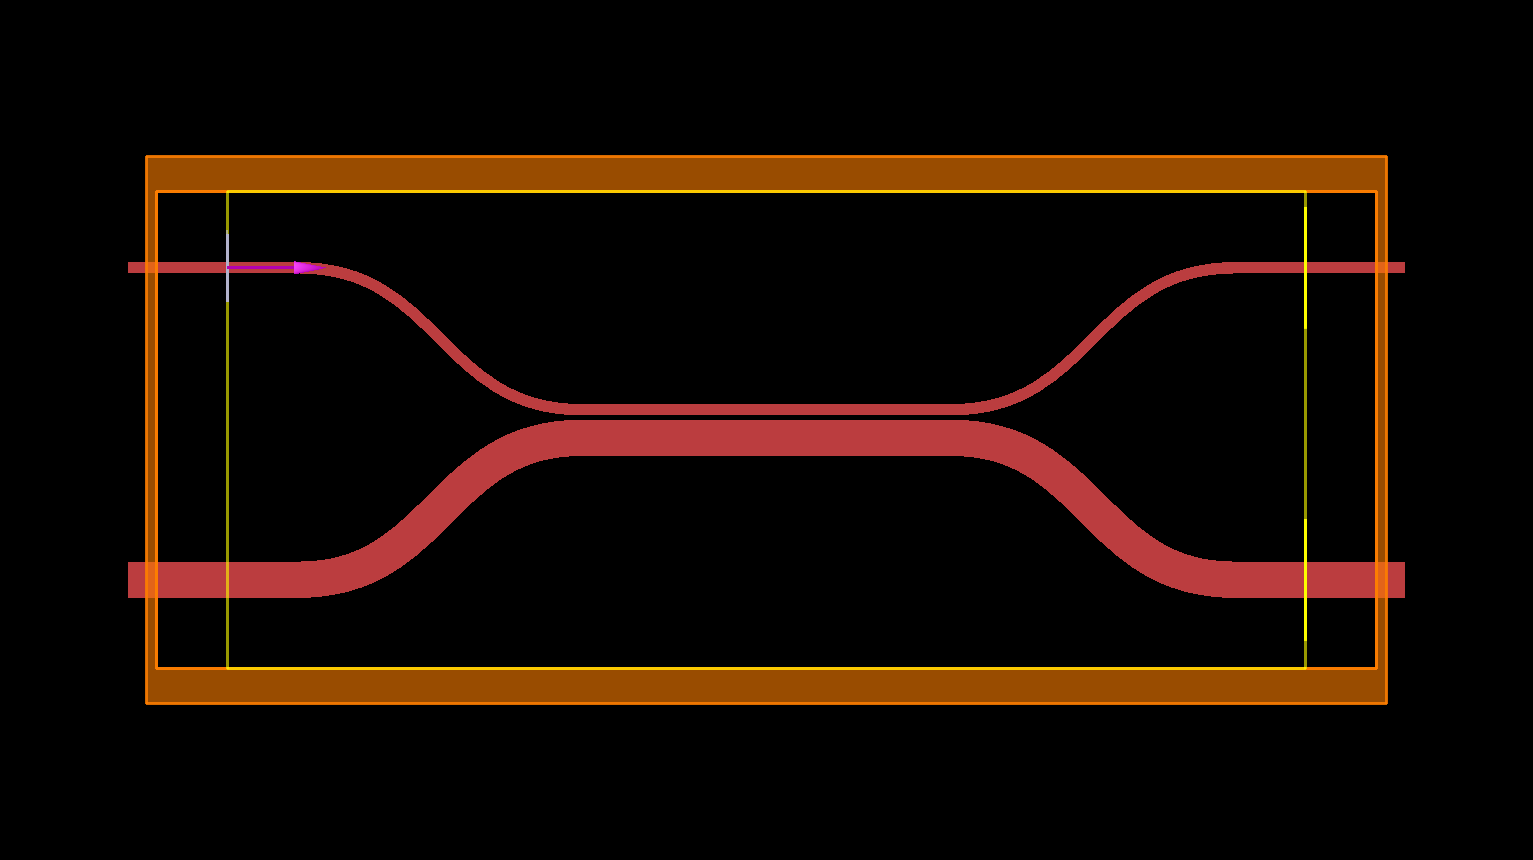
\includegraphics[width=0.8\textwidth]{task3/views/wg1_width=0.4_wg2_width=1.28_separation=0.15_coupling_length=13.0.png}
  \caption{Schematic of the S-bend directional coupler geometry
  with parameters \(w_1=\SI{400}{\nm}\), \(w_2=\SI{1280}{\nm}\), \(\text{separation}=\SI{150}{\nm}\), and \(L=\SI{13.0}{\um}\).}
  \label{fig:s_bend_coupler}
\end{figure}

\section{Results}

Throughout this section, graphs and figures may reference the quantities \texttt{T\_net\_br} (abbreviated to \texttt{br}) and \texttt{T\_net\_tr} (abbreviated to \texttt{tr}),
which are the total power transfer fraction to the lower waveguide TE\textsubscript{0} mode monitor and the upper waveguide TE\textsubscript{0} mode monitor respectively.

\subsection{TE\textsubscript{0}-TE\textsubscript{0} coupling}

For equal waveguide widths, it is quite straightforward to achieve arbitrary TE\textsubscript{0}-TE\textsubscript{0} power transfer between the two coupled waveguides.
The fundamental principle enabling efficient power transfer between two modes is the phase matching condition,
which dictates that their propagation constants, \(\beta_1\) and \(\beta_2\), must be closely matched, i.e., the phase mismatch \(\Delta\beta = \beta_1 - \beta_2 \approx 0\).
Since the propagation constant is related to the effective index \(n_\text{eff}\) by \(\beta = k_0 n_\text{eff}\), where \(k_0 = 2\pi/\lambda\) is the free-space wavenumber,
this condition implies that their effective indices must be nearly equal: \(n_{\text{eff},1} \approx n_{\text{eff},2}\).
With TE\textsubscript{0} launched at the input port of the upper waveguide, an identically dimensioned co-located waveguide (symmetrised across the separation gap) supports a TE\textsubscript{0} mode with the same effective index
(subject to fabrication tolerances), thus inherently satisfying the phase matching condition.
Consequently, the TE\textsubscript{0} mode of the upper waveguide is efficiently coupled to the TE\textsubscript{0} mode of the lower waveguide.

Other modes, such as higher-order TE modes (TE\textsubscript{1}, TE\textsubscript{2}, etc.) or TM modes, generally have significantly different effective indices compared to the TE\textsubscript{0} mode in the same waveguide geometry.
This results in a large phase mismatch \(\Delta\beta=k_0\Delta n_\text{eff}\gg 1\) with respect to TE\textsubscript{0}.
The power transfer amplitude \(A\) between two modes over a length \(L\) with coupling coefficient \(\kappa\) is proportional to \(\frac{\kappa^2}{\kappa^2 + {(\Delta\beta/2)}^2}\).
Hence, for large \(\Delta\beta\), cross-mode leakage has a negligible modal power beating amplitude of
\[A\propto\frac{\kappa^2}{\kappa^2+{(\frac{\Delta\beta}{2})}^2}\approx{\left(\frac{2\kappa}{\Delta\beta}\right)}^2\to 0.\]

Moreover, by selecting the waveguide width \(w\) to be sufficiently small, specifically below the cutoff width for these higher-order modes, they become non-propagating (evanescent) and cannot effectively guide light or participate significantly in the coupling process.
The cutoff condition for a mode occurs when its effective index \(n_\text{eff}\) approaches the refractive index of the cladding material \(n_\text{clad}\).

Assuming phase matching (\(\Delta\beta=0\)) and input power \(P_1(0)\) in the first waveguide, the power transferred \(P_2(L)\) to the second (initially unexcited) waveguide as a function of the coupling length \(L\) is given by
\[
P_2(L) = P_1(0)\sin^2(\kappa L),
\]
where \(\kappa\) is the coupling coefficient. This coefficient quantifies the strength of the interaction between the evanescent fields of the modes in the two waveguides and is a function of the waveguide geometry (widths, separation gap), material properties, and wavelength.

\paragraph{Power transfer as a function of coupling length}
Figure~\ref{fig:coupling_length} shows the power transfer as a function of the coupling length \(L\) for a fixed waveguide width of \SI{500}{\nm} and separation gap of \SI{150}{\nm},
with the TE\textsubscript{0} mode launched at a wavelength of \SI{1550}{\nm} from the input port of the upper waveguide.
The coupled mode theory predicts sinusoidal power beating. Half-power transfer (\(P_2(L_{3\text{dB}}) = P_1(0)/2\)) occurs when \(\kappa L_{3\text{dB}} = \pi/4\), so the minimum coupling length for this is \(L_{3\text{dB}}=\frac{\pi}{4\kappa}\).
Total power transfer (\(P_2(L_c) = P_1(0)\)) occurs when \(\kappa L_c = \pi/2\), so the minimum coupling length for this is \(L_c=\frac{\pi}{2\kappa}\).
Indeed, we observe \(\hat{L}_{3\text{dB}}\approx\SI{10}{\um}\) and \(\hat{L}_c\approx\SI{21}{\um}\) in the simulation results.


\begin{figure}[h!]
  \centering
  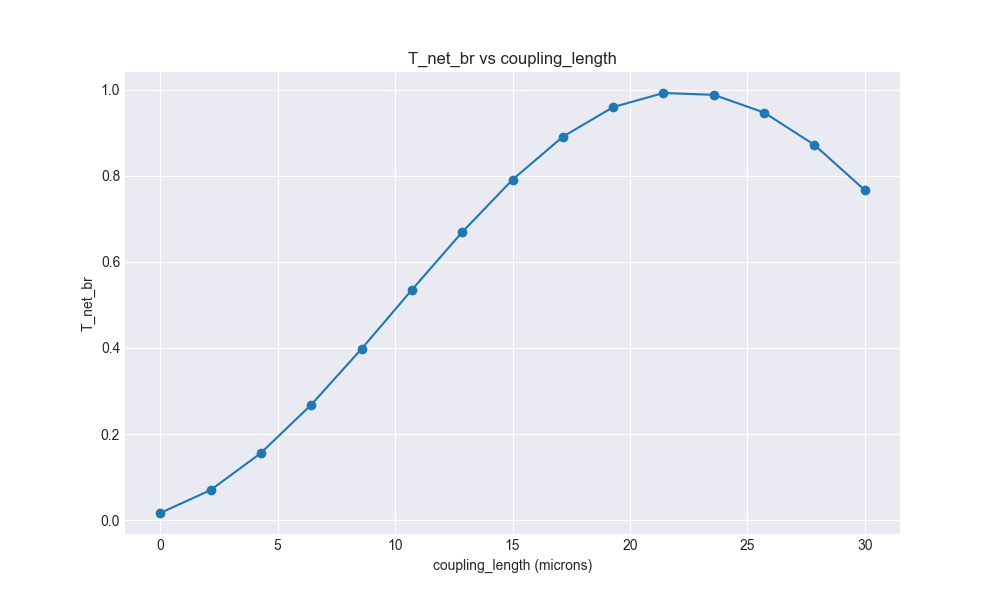
\includegraphics[width=0.8\textwidth]{task3/sweep_plots/sweep_idx_0_sweep__coupling_length=0_30_15_T_net_br_line.png}
  \caption{Cross-power transfer fraction at the coupled output port as a function of coupling length \(L\) for a fixed waveguide width of \SI{500}{\nm} and separation gap of \SI{150}{\nm} under input port TE\textsubscript{0} mode excitation at \SI{1550}{\nm}.}
  \label{fig:coupling_length}
\end{figure}


\paragraph{Half-power transfer}
Figure~\ref{fig:eq_power_distribution} shows the power intensity distribution across the waveguide plane
for the half-power simulation at \(\hat{L}_{3\text{db}}\approx\SI{10}{\um}\).
The TE\textsubscript{0} mode monitor registers a power transfer fraction of
\(0.5056\) while the lower waveguide TE\textsubscript{0} mode monitor registers a power transfer fraction of
\(0.4895\). This implies some power loss, but higher-order mode monitors
show that either the mode is not supported, or that the power transfer fraction is negligible.

\begin{figure}[h!]
  \centering
  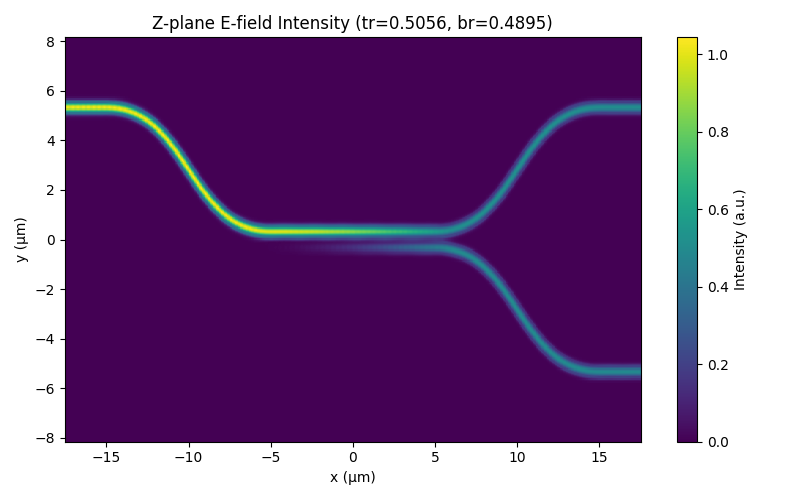
\includegraphics[width=0.8\textwidth]{task3/sim_1742_110625/z_plane_intensity.png}
  \caption{Power intensity distribution across the waveguide plane at the half-power coupling length \(\hat{L}_{3\text{db}}\approx\SI{10}{\um}\) for a fixed waveguide width of \SI{500}{\nm} and separation gap of \SI{150}{\nm} under input port TE\textsubscript{0} mode excitation at \SI{1550}{\nm}.}
  \label{fig:eq_power_distribution}
\end{figure}

\paragraph{Total power transfer}
Figure~\ref{fig:max_power_distribution} shows the power intensity distribution across the waveguide plane
for the total power transfer simulation at \(\hat{L}_c\approx\SI{21}{\um}\).
With cross-mode power transfer to the lower waveguide TE\textsubscript{0} mode monitor registering a power transfer fraction of
\(0.9920\), we can conclude that the upper TE\textsubscript{0} mode is indeed coupled strongly to the lower waveguide TE\textsubscript{0} mode.
This latter parameter set gives us an optimised directional coupler operating at \(\lambda=\SI{1550}{\nm}\).

It should be noted that such a small separation gap utilised above is the minimum of what is achievable in practice,
and in the next section we will explore the effect of varying the separation gap on the power transfer fraction.

\begin{figure}[h!]
  \centering
  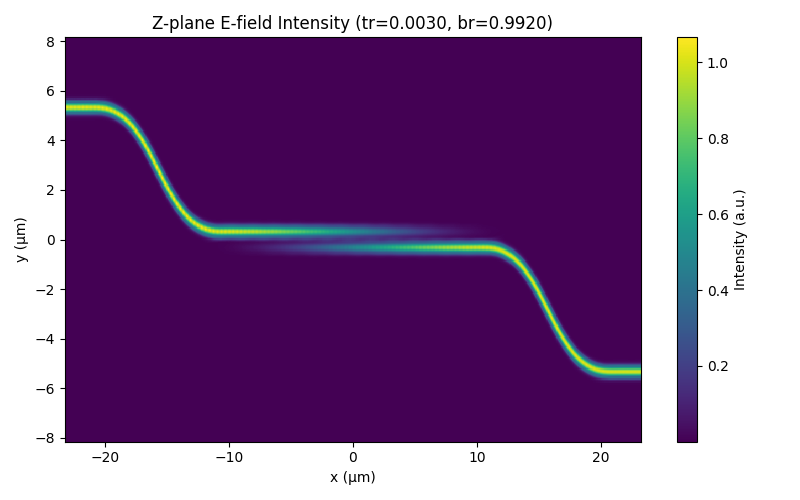
\includegraphics[width=0.8\textwidth]{task3/sim_2318_110625/z_plane_intensity.png}
  \caption{Power intensity distribution across the waveguide plane at the total power transfer coupling length \(\hat{L}_c\approx\SI{21}{\um}\) for a fixed waveguide width of \SI{500}{\nm} and separation gap of \SI{150}{\nm} under input port TE\textsubscript{0} mode excitation at \SI{1550}{\nm}.}
  \label{fig:max_power_distribution}
\end{figure}

\paragraph{Optimising for a shorter wavelength}
To additionally optimise a directional coupler for a shorter wavelength \(\lambda=\SI{1310}{\nm}\), we could repeat the above procedure with the same fixed waveguide width of \SI{500}{\nm} and separation gap of \SI{150}{\nm}.
However, a shorter wavelength generally requires a larger coupling length to achieve the same fraction of power transfer, or a modification of the waveguide geometry.
The coupling coefficient \(\kappa\) is wavelength-dependent. For a fixed geometry, as \(\lambda\) decreases, a guided mode tends to become more confined within the waveguide core. This increased confinement reduces the extent of its evanescent field into the cladding and, consequently, into the adjacent waveguide. A reduced evanescent field overlap leads to a smaller \(\kappa\). Since the coupling length for total power transfer \(L_c = \frac{\pi}{2\kappa}\), a smaller \(\kappa\) necessitates a larger \(L_c\).
Furthermore, the phase mismatch \(\Delta\beta = k_0 \Delta n_\text{eff} = \frac{2\pi}{\lambda} \Delta n_\text{eff}\) becomes more sensitive to any small inherent or fabrication-induced differences in \(n_\text{eff}\) at shorter wavelengths, potentially diminishing coupling efficiency if \(n_\text{eff}\) is not perfectly matched.

Figure~\ref{fig:coupling_length_1310} shows the power transfer as a function of the coupling length \(L\) for a fixed waveguide width of \SI{500}{\nm} and separation gap of \SI{150}{\nm} over the same swept range as before,
and within this range, we cannot even achieve half-power transfer,
let alone total power transfer. It seems that either we need to have a very large coupling length,
or to modify the waveguide geometry.

\begin{figure}[h!]
  \centering
  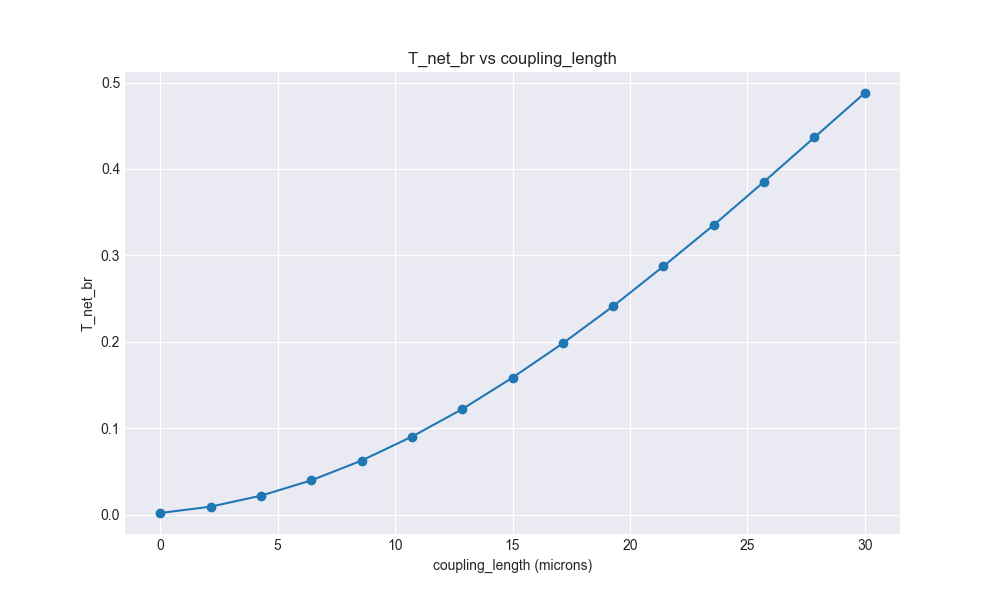
\includegraphics[width=0.8\textwidth]{task3/sweep_plots/sweep_idx_1_sweep__coupling_length=0_30_15,_center_wavelength=1.31_T_net_br_line.png}
  \caption{Cross-power transfer fraction at the coupled output port as a function of coupling length \(L\) for a fixed waveguide width of \SI{500}{\nm} and separation gap of \SI{150}{\nm} under input port TE\textsubscript{0} mode excitation at \SI{1310}{\nm}.}
  \label{fig:coupling_length_1310}
\end{figure}

\paragraph{Reducing the coupling length}
Assuming fabrication tolerances are not a concern
and we do not require the dimensions of the directional coupler to match other components in the photonic circuit, like cascaded couplers or integrated Michelson interferometers, it is desireable to reduce the coupling length.
Shorter directional couplers have a smaller footprint,
less propagation loss (as loss is proportional to length) and latency,
and often support a broader spectral bandwidth because the phase accumulation \(\kappa L\) is less sensitive to changes in \(\kappa(\lambda)\) if \(L\) is small.
Additionally they are more robust against accumulated phase mismatch \(\Delta\beta L\) arising from non-idealities in the fabrication process.

One strategy to achieve this for our directional coupler at \(\lambda=\SI{1310}{\nm}\) is to use the fact that decreasing the waveguide width (while ensuring the mode remains well-guided and above cutoff) increases the lateral evanescent extent of the modes.
This is because a narrower core provides weaker confinement. The increased overlap of these more extensive evanescent fields between the two waveguides leads to a stronger interaction, and thus a larger coupling coefficient \(\kappa\). Since the coupling length for total power transfer \(L_c = \frac{\pi}{2\kappa}\), a larger \(\kappa\) results in a shorter \(L_c\).

By reducing the waveguide width to \SI{400}{\nm}, we can achieve Figure~\ref{fig:coupling_length_1310_w400},
which shows that we can achieve half-power transfer at \(\hat{L}_{3\text{db}}\approx\SI{11}{\um}\) and total power transfer at \(\hat{L}_c\approx\SI{23}{\um}\). This is much more comparable to the \(\hat{L}_{3\text{db}}\approx\SI{10}{\um}\) and \(\hat{L}_c\approx\SI{21}{\um}\) for the \SI{1550}{\nm} wavelength case with a \SI{500}{\nm} waveguide width.

\begin{figure}[h!]
  \centering
  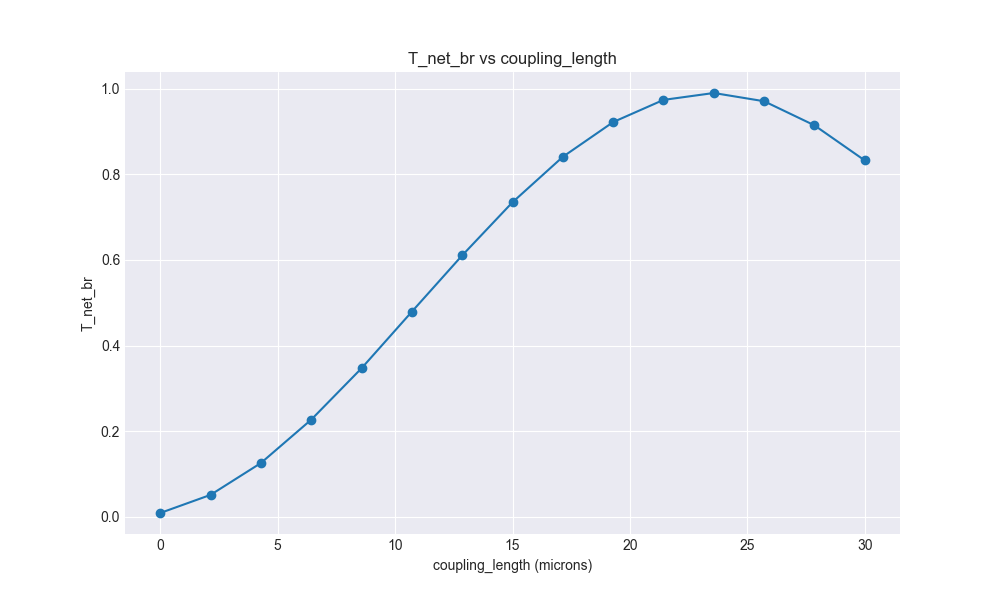
\includegraphics[width=0.8\textwidth]{task3/sweep_plots/sweep_idx_6_sweep__coupling_length=0_30_15_wg1_width=0.4_wg2_width=0.4_separation=0.15_center_wavelength=1.31_T_net_br_line.png}
  \caption{Cross-power transfer fraction at the coupled output port as a function of coupling length \(L\) for a fixed waveguide width of \SI{400}{\nm} and separation gap of \SI{150}{\nm} under input port TE\textsubscript{0} mode excitation at \SI{1310}{\nm}.}
  \label{fig:coupling_length_1310_w400}
\end{figure}

\subsection{Effect of waveguide width and separation gap}

It is not always so trivial to design a directional coupler that achieves the desired operation characteristics,
hence it is useful to explore the effect of the hyperparameters fixed before optimised over the coupling length \(L\),
namely the waveguide width and separation gap.

Figure~\ref{fig:2D_sweep_equal_wg_vs_sep} shows the power transfer fraction to the lower waveguide TE\textsubscript{0} mode monitor
as a function of the uniform waveguide width \(w\) swepth through \(w\in[0.1, 1.0]\,\unit{\um}\) and separation gap \(s\) swept through \(s\in[0.15, 0.5]\,\unit{\um}\) for a fixed coupling length of \SI{10}{\um} and input port TE\textsubscript{0} mode excitation at \SI{1550}{\nm}. For the majority of the parameter space, there is very weak coupling.
However, we observe a ridge of strong power transfer along the entire separation axis at a waveguide width of \(w=\SI{0.36}{\um}\),
with a peak at \(s=\SI{0.25}{\um}\).

\begin{figure}[h!]
  \centering
  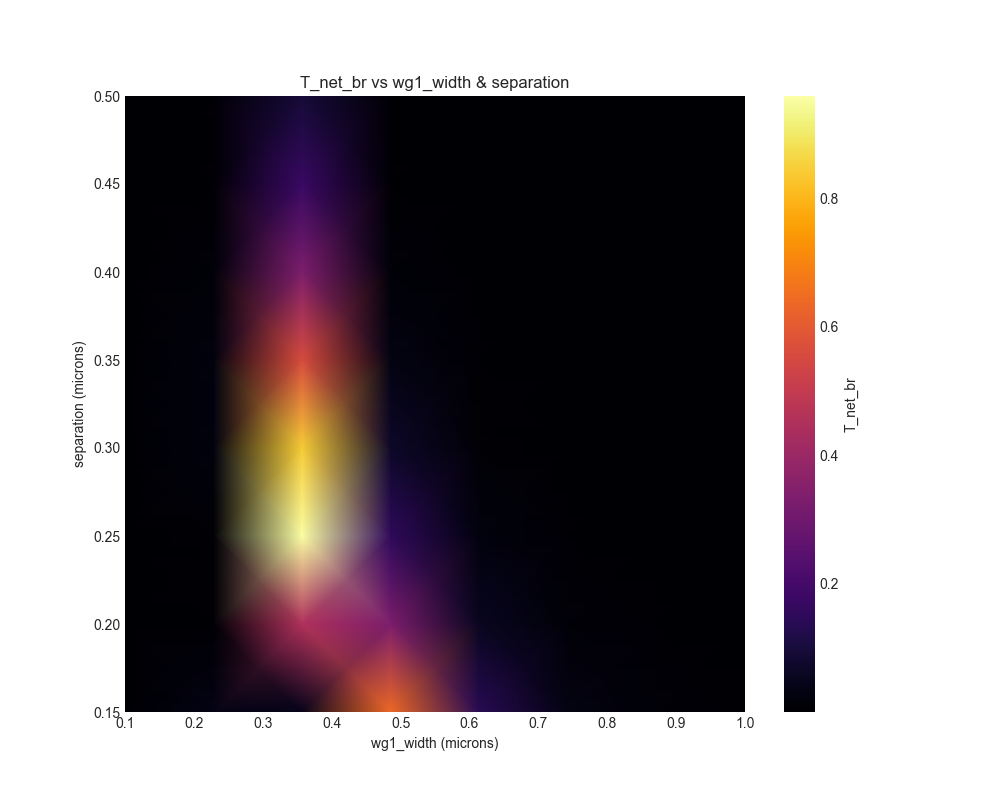
\includegraphics[width=0.8\textwidth]{task3/sweep_plots/sweep_idx_2_sweep__wg1_width=0.1_1_8,_wg2_width=0.1_1_8,_separation=0.15_0.5_8_(matched_widths)_T_net_br_heatmap.png}
  \caption{Cross-power transfer fraction at the coupled output port as a function of waveguide width \(w\) and separation gap \(s\) for a fixed coupling length of \SI{10}{\um} under input port TE\textsubscript{0} mode excitation at \SI{1550}{\nm}.}
  \label{fig:2D_sweep_equal_wg_vs_sep}
\end{figure}

\paragraph{Effect of waveguide width}
While a small waveguide width \(w\) increases the evanescent overlap (enhancing \(\kappa\)),
it also reduces the mode confinement. As \(w\) decreases and approaches the cutoff width, the effective index \(n_\text{eff}\) of the mode approaches the refractive index of the cladding \(n_\text{clad}\).
This weak confinement makes the mode highly susceptible to bending-induced radiative losses, particularly in the S-bend sections of the coupler. The bending loss coefficient \(\alpha_b\) typically increases exponentially as \(n_\text{eff}\) approaches \(n_\text{clad}\)\autocite{sakaiSimplifiedBendingLoss1979}.
Figure~\ref{fig:high_bend_loss} shows the power intensity distribution across the waveguide plane
for a waveguide width just before the ridge \(w=\SI{0.23}{\um}\) and at the optimal separation gap \(s=\SI{0.25}{\um}\).

From this it is clear that the mode is not well confined, and loses almost all of its power along the input port S-bend.

\begin{figure}[h!]
  \centering
  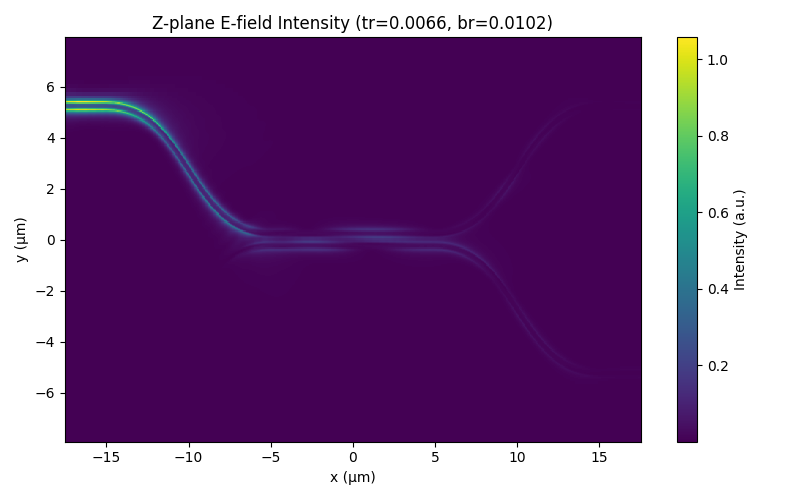
\includegraphics[width=0.8\textwidth]{task3/sim_0524_120625/z_plane_intensity.png}
  \caption{Power intensity distribution across the waveguide plane at the coupling length \(L=\SI{10}{\um}\) for a waveguide width of \(w=\SI{0.23}{\um}\) and separation gap of \(s=\SI{0.25}{\um}\) under input port TE\textsubscript{0} mode excitation at \SI{1550}{\nm}.}
  \label{fig:high_bend_loss}
\end{figure}

Very large waveguide widths, on the other hand, provide much stronger mode confinement, meaning \(n_\text{eff}\) is significantly larger than \(n_\text{clad}\) and approaches the core index \(n_\text{core}\).
This results in a smaller evanescent tail extending into the cladding, which reduces the coupling coefficient \(\kappa\). For a fixed coupling length \(L\), a smaller \(\kappa\) leads to a smaller power transfer fraction \(\sin^2(\kappa L)\).
(One could increase \(L\) to compensate for a smaller \(\kappa\), but in Figure~\ref{fig:2D_sweep_equal_wg_vs_sep}, \(L\) was held constant.)
The optimal waveguide width is thus a balance between these two effects: achieving sufficient evanescent field overlap for strong coupling (favoring smaller \(w\)) while maintaining strong enough mode confinement to minimize propagation and bending losses (favoring larger \(w\)).
The observed ridge of strong power transfer at \(w=\SI{0.36}{\um}\) is the result of this trade-off for the given \(L=\SI{10}{\um}\).

\paragraph{Effect of separation gap}

Now that we have established the optimal waveguide width for a fixed \(L\),
in analysis of the separation gap \(s\), it may be more intuitive to fix the width at this optimum (\(w \approx \SI{0.36}{\um}\)) and consider the effect of separation on the ridge profile,
which is shown in Figure~\ref{fig:coupled_power_ridge}.
At a large separation, the power transfer fraction decays, which is expected as the coupling coefficient \(\kappa\) typically exhibits an approximately exponential dependence on \(s\), i.e., \(\kappa \propto e^{-\gamma s}\), where \(\gamma\) is related to the decay constant of the evanescent field in the cladding\autocite{dolph5CharacteristicsEvanescent2025}. Thus, as \(s\) increases, \(\kappa\) decreases significantly, leading to reduced power transfer for a fixed \(L\).
However, at a very small separation, the power transfer fraction is also small and appears to increase with the separation gap initially.

% TODO: rigorously mathematically justify the exponential decay and linear increase
% Is the linear increase due to some cancellation? Or possibly due to some quantity being very large? Does it come out in a Taylor expansion?

The former (decay at large \(s\)) can be rationalised by the fact that the evanescent tails of the modes in each waveguide overlap less and less as the separation gap increases.
The latter behaviour (increase from very small \(s\)) is less immediately intuitive but can be understood by considering the \(\sin^2(\kappa L)\) dependence.
At very small separation \(s\), the two waveguides become very strongly coupled, and the system is better described by its supermodes (even and odd symmetric modes for identical waveguides). The propagation constants of these supermodes, \(\beta_e\) and \(\beta_o\), become significantly different, and the coupling coefficient \(\kappa = |\beta_e - \beta_o|/2\) becomes large.
If \(L\) is fixed (here, \(L=\SI{10}{\um}\)), and \(\kappa\) is very large due to small \(s\), the argument \(\kappa L\) might be significantly greater than \(\pi/2\) (the first maximum for \(\sin^2(\kappa L)\)). For instance, if \(\kappa L\) is close to \(\pi\), the power transfer would be close to zero. As \(s\) increases slightly from its minimum, \(\kappa\) decreases. This decrease in \(\kappa\) could bring \(\kappa L\) closer to \(\pi/2\) (or \(3\pi/2\), etc.), thereby increasing the power transfer \(\sin^2(\kappa L)\).
The peak in Figure~\ref{fig:coupled_power_ridge} at \(s=\SI{0.25}{\um}\) corresponds to the separation where \(\kappa(w=\SI{0.36}{\um}, s)L \approx \pi/2\) (or more generally, \((m+1/2)\pi\) for integer \(m\)).
Indeed, Figure~\ref{fig:2D_sweep_equal_wg_vs_sep} shows that for very small separations,
the ridge of strong cross-power transfer moves diagonally towards larger waveguide widths.
This is because, for a fixed coupling length \(L\), as \(s\) decreases (which tends to increase \(\kappa\)), \(w\) must increase (which tends to decrease \(\kappa\) by increasing confinement) to maintain the condition \(\kappa(w,s) L \approx (m+1/2)\pi\) for optimal power transfer.

\begin{figure}[h!]
  \centering
  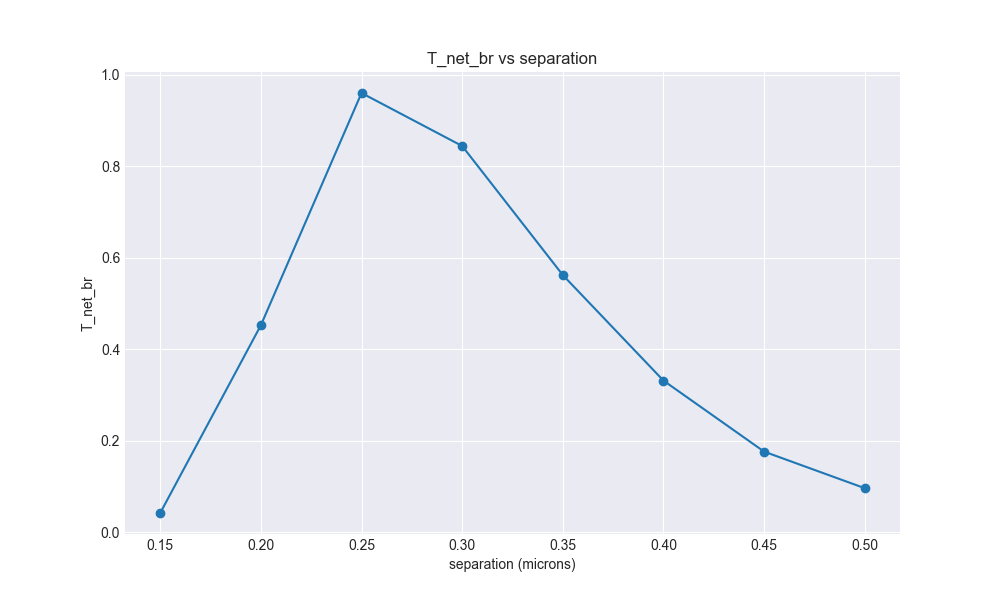
\includegraphics[width=0.8\textwidth]{task3/sweep_plots/sweep_idx_10_sweep__coupling_length=10_wg1_width=0.3571428571428572_wg2_width=0.3571428571428572_separation=0.15_0.5_8_center_wavelength=1.55_T_net_br_line.png}
  \caption{Cross-power transfer fraction at the coupled output port as a function of separation gap \(s\) for a fixed waveguide width of \(w=\SI{0.36}{\um}\) under input port TE\textsubscript{0} mode excitation at \SI{1550}{\nm}.}
  \label{fig:coupled_power_ridge}
\end{figure}

\subsection{Cross-order mode coupling}

Designing for coupling across modes of different orders is less trivial. 
For the TE\textsubscript{0}-TE\textsubscript{0} case we were able to rely on the fact that equal waveguide widths impose TE\textsubscript{0} phase matching across the separation gap,
but this is not the case for general cross-order mode coupling.
The primary condition for efficient coupling between mode \(m\) in waveguide 1 (width \(w_1\)) and mode \(n\) in waveguide 2 (width \(w_2\)) is phase matching: \(\beta_{1,m} \approx \beta_{2,n}\), which translates to \(n_{\text{eff},1,m}(w_1, \lambda) \approx n_{\text{eff},2,n}(w_2, \lambda)\).

% I chose TE0-TE2
% TODO: rigorously show whether TE0-TE1 is possible, or if parity forbids it / requires lateral displacement of the 2nd waveguide
% Specifically for the geometry described above.
% Need to justify the choice of TE\textsubscript{0}-TE\textsubscript{2} coupling.
Coupling between modes of different parity, such as TE\textsubscript{0} (even transverse field symmetry) and TE\textsubscript{1} (odd transverse field symmetry), is generally forbidden or very weak in symmetric directional couplers where the waveguides are aligned (no lateral offset). This is because the coupling coefficient \(\kappa\) involves an overlap integral of the mode fields. If the product of the fields has odd symmetry with respect to the center of the coupling region, the integral evaluates to zero.
TE\textsubscript{2}, like TE\textsubscript{0}, possesses an even transverse field symmetry (for its dominant E-field component), allowing for a non-zero overlap integral and thus potentially strong coupling if phase matching is achieved.

There is an additional step of design required to achieve cross-order mode coupling:
engineering the waveguide dimensions (typically their widths, \(w_1\) and \(w_2\)) to match the effective indices of the two desired modes across the separation gap at the operating wavelength.

\paragraph{TE\textsubscript{0}-TE\textsubscript{2} coupling}
Let us consider the example of designing a directional coupler that transfers maximum power from the TE\textsubscript{0} mode of the upper waveguide (width \(w_1\)) to the TE\textsubscript{2} mode of the lower waveguide (width \(w_2\)).
To achieve phase matching, \(n_{\text{eff,TE0}}(w_1, \lambda) \approx n_{\text{eff,TE2}}(w_2, \lambda)\).
Since higher-order modes generally have lower effective indices than lower-order modes in waveguides of the same width, achieving this condition typically requires \(w_2 > w_1\) if both waveguides are made of the same core and cladding materials. This is because \(n_\text{eff}\) for any given guided mode generally increases with waveguide width (for a mode well above cutoff).
Recall Figure~\ref{fig:te_neff} from the first interim report\autocite{ngSB4IntegratedPhotonics2025}.
This idealised planar waveguide case demonstrates that we expect that,
with the upper waveguide width fixed at \(w_1=\SI{0.4}{\um}\) (supporting primarily TE\textsubscript{0}),
it should be possible to couple to the TE\textsubscript{2} mode of the lower waveguide when its width \(w_2\) is significantly larger, such that \(n_{\text{eff,TE2}}(w_2)\) matches \(n_{\text{eff,TE0}}(w_1)\).
The plot suggests that for \(n_{\text{eff,TE0}}(w_1=\SI{0.4}{\um})\), a matching \(n_{\text{eff,TE2}}(w_2)\) might occur for \(w_2\) in the range of \(1\,\unit{\um}\) to \(1.5\,\unit{\um}\).

\begin{figure}[h!]
  \centering
  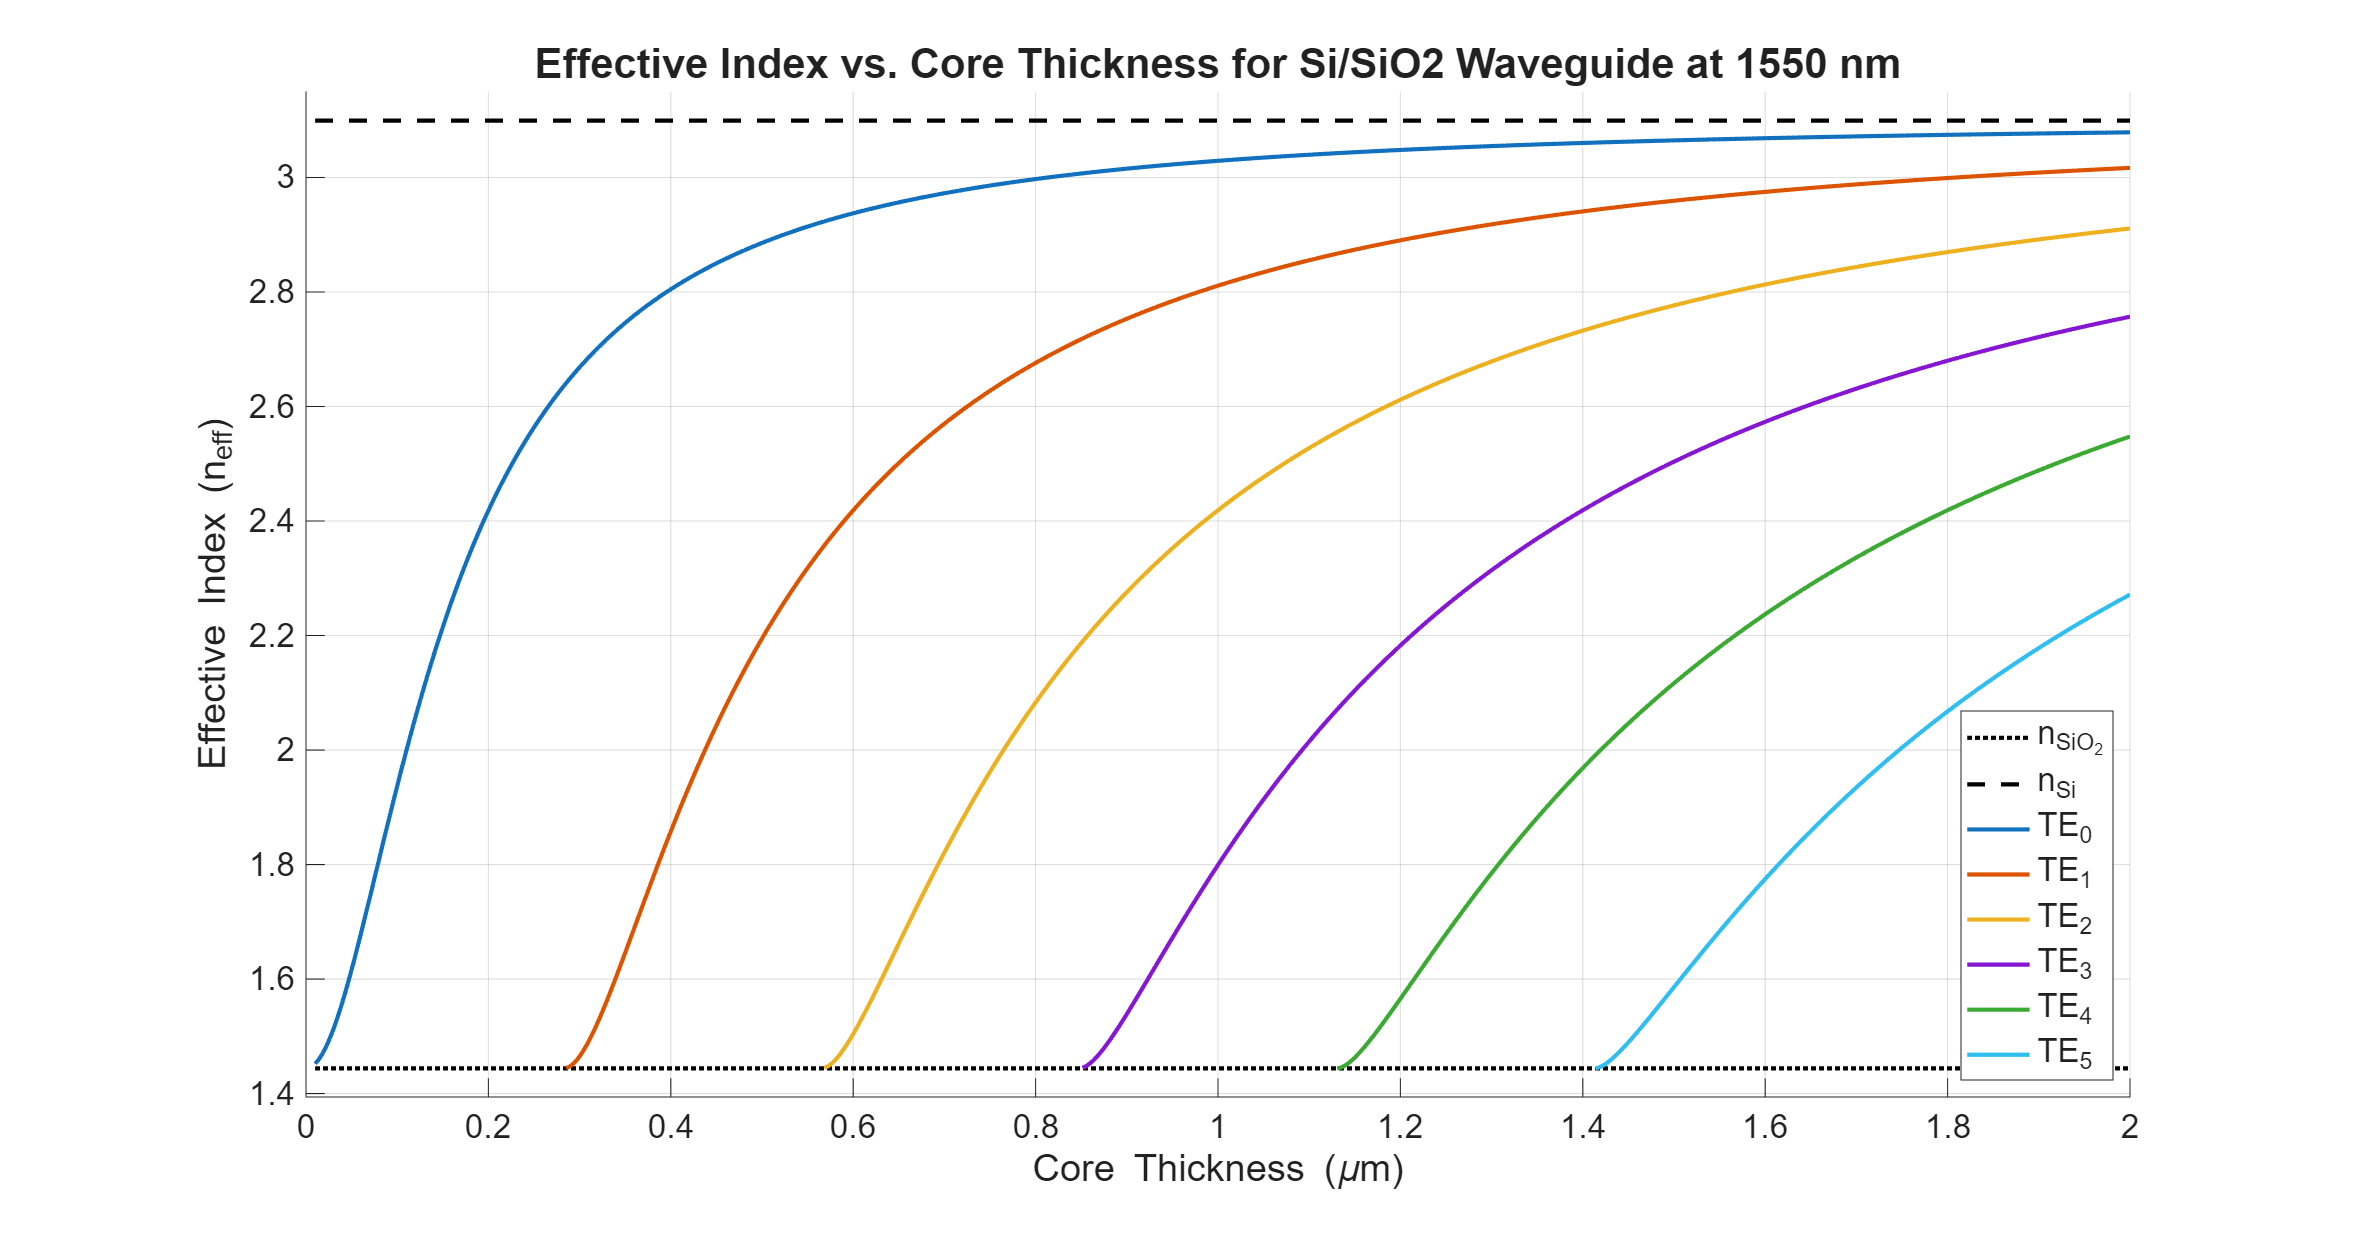
\includegraphics[width=0.8\textwidth]{task1/neff_vs_thickness_Si_SiO2_1550nm.png}
  \caption{Effective indices of TE\textsubscript{0}-TE\textsubscript{5} as a function of waveguide thickness.}
  \label{fig:te_neff}
\end{figure}

To avoid adding additional monitors to the simulation sweep,
it will suffice to use the upper output port TE\textsubscript{0} mode monitor as an inverse proxy for the lower output port TE\textsubscript{2} mode monitor. That is, minimizing power remaining in the TE\textsubscript{0} mode of the input waveguide implies maximizing power transferred to other phase-matched modes (hopefully the desired TE\textsubscript{2} mode in the other waveguide, assuming other couplings are weak or non-phase-matched).
One design strategy is to sweep both the lower waveguide width \(w_2\) through the range \(w_2\in(1,1.5]\,\unit{\um}\) and the coupling length \(L\in[10,40]\,\unit{\um}\) while keeping the separation gap fixed at \(s=\SI{0.15}{\um}\).
This produces the heatmap in Figure~\ref{fig:te0_te2_coupling_heatmap} of the power fraction received by the proxy TE\textsubscript{0} mode monitor on the upper waveguide.
\begin{figure}[h!]
  \centering
  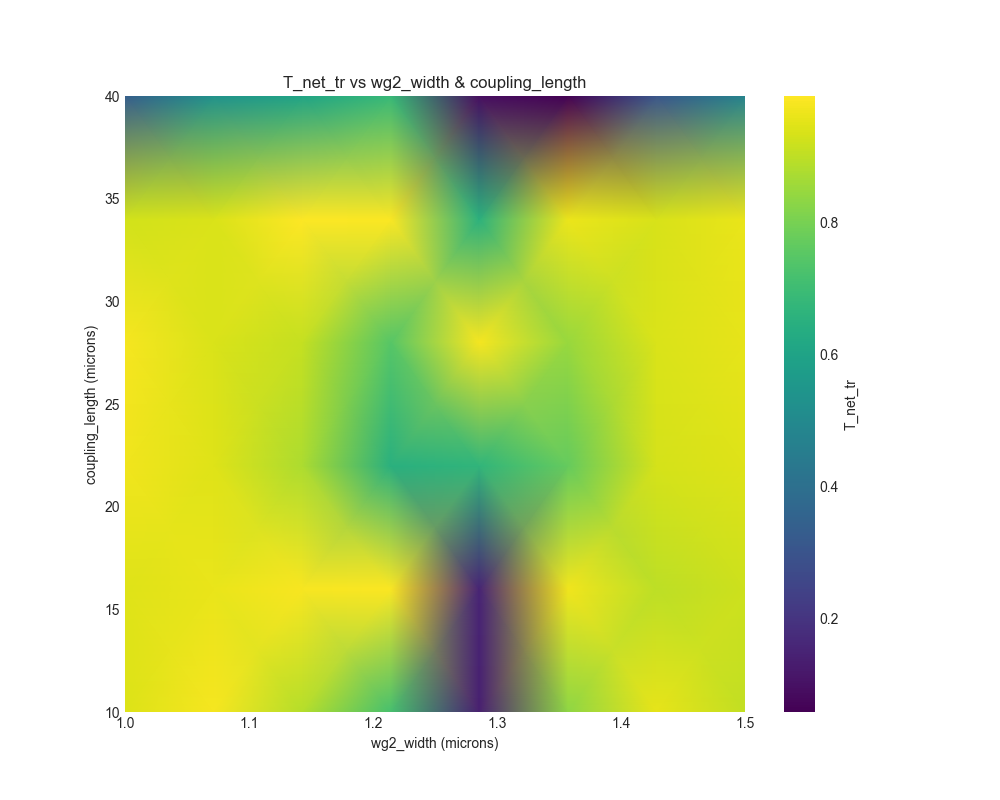
\includegraphics[width=0.8\textwidth]{task3/sweep_plots/sweep_idx_7_sweep__coupling_length=10_40_6_wg1_width=0.4_wg2_width=1_1.5_8_separation=0.15_center_wavelength=1.55_T_net_tr_heatmap.png}
  \caption{Cross-power transfer fraction at the upper waveguide TE\textsubscript{0} mode monitor as a function of lower waveguide width \(w_2\) and coupling length \(L\) for a fixed upper waveguide width of \(w_1=\SI{0.4}{\um}\) and separation gap of \(s=\SI{0.15}{\um}\) under input port TE\textsubscript{0} mode excitation at \SI{1550}{\nm}.}
  \label{fig:te0_te2_coupling_heatmap}
\end{figure}

Clearly, we have a sinusoidal ridge of recorded power transfer (more accurately, power \textit{not} transferred away from the input TE\textsubscript{0} mode)
along the coupling length axis,
at a waveguide width of \(w_2=\SI{1.28}{\um}\). This \(w_2\) value is where phase matching \(n_{\text{eff,TE0}}(w_1=\SI{0.4}{\um}) \approx n_{\text{eff,TE2}}(w_2=\SI{1.28}{\um})\) is best achieved.
Fixing that width and looking along at ridge results in Figure~\ref{fig:te0_te2_coupling_length}, showing the optimum coupling length \(L\) for maximum power transfer to the TE\textsubscript{2} mode of the lower waveguide (indicated by minimum power remaining in the upper TE\textsubscript{0} mode)
to be \(\hat{L}\approx\SI{13}{\um}\). Figure~\ref{fig:cross_mode_power_distribution} shows the power intensity distribution across the waveguide plane at this coupling length,
with the TE\textsubscript{0} mode monitor on the upper waveguide registering a power transfer fraction of \(0.0182\) with \(n_\text{eff}=2.217\) and the TE\textsubscript{2} mode monitor (the third mode filtered by TE/TM fraction in Lumerical) on the lower waveguide registering a power transfer fraction of \(0.9235\) with \(n_\text{eff}=2.223\). The close matching of these effective indices confirms the phase matching condition. This means the TE\textsubscript{2} mode is excited to approximately \(0.9235 / (0.9235 + 0.0182) \approx 98.1\%\) of the total power detected in these two specific modes at the output. There is some launched power unaccounted for (\(1 - 0.0182 - 0.9235 = 0.0583\), or about \(5.8\%\)), which can be attributed to radiation losses (e.g., at S-bends), coupling to other non-monitored modes, or scattering.

This is the directional coupler shown originally in Figure~\ref{fig:s_bend_coupler}.

\begin{figure}[h!]
  \centering
  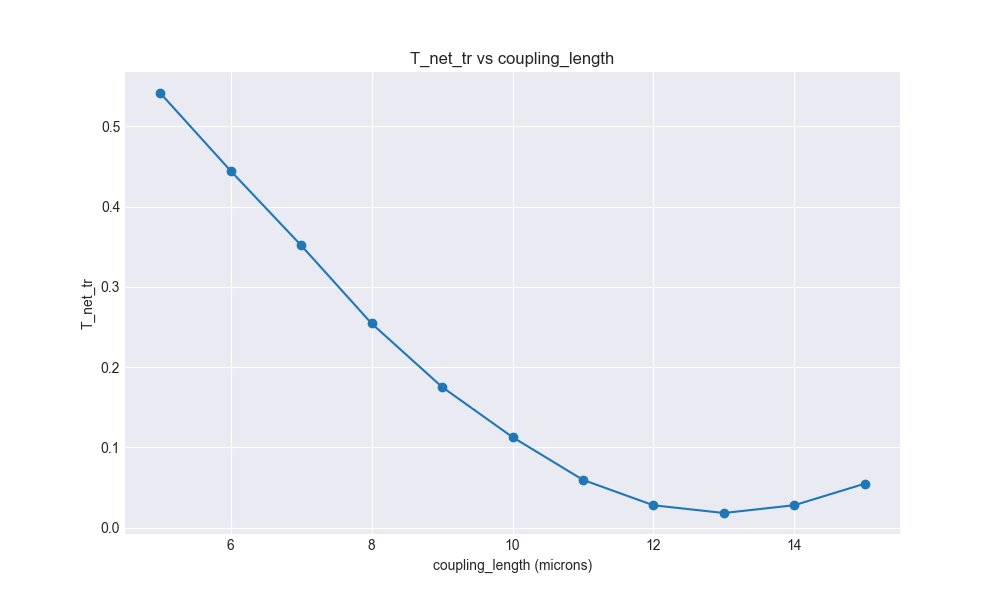
\includegraphics[width=0.8\textwidth]{task3/sweep_plots/sweep_idx_8_sweep__coupling_length=5_15_11_wg1_width=0.4_wg2_width=1.28_separation=0.15_center_wavelength=1.55_T_net_tr_line.png}
  \caption{Power transfer fraction at the upper waveguide TE\textsubscript{0} mode monitor as a function of coupling length \(L\) for a fixed upper waveguide width of \(w_1=\SI{0.4}{\um}\), lower waveguide width of \(w_2=\SI{1.28}{\um}\), and separation gap of \(s=\SI{0.15}{\um}\) under input port TE\textsubscript{0} mode excitation at \SI{1550}{\nm}.}
  \label{fig:te0_te2_coupling_length}
\end{figure}
\begin{figure}[h!]
  \centering
  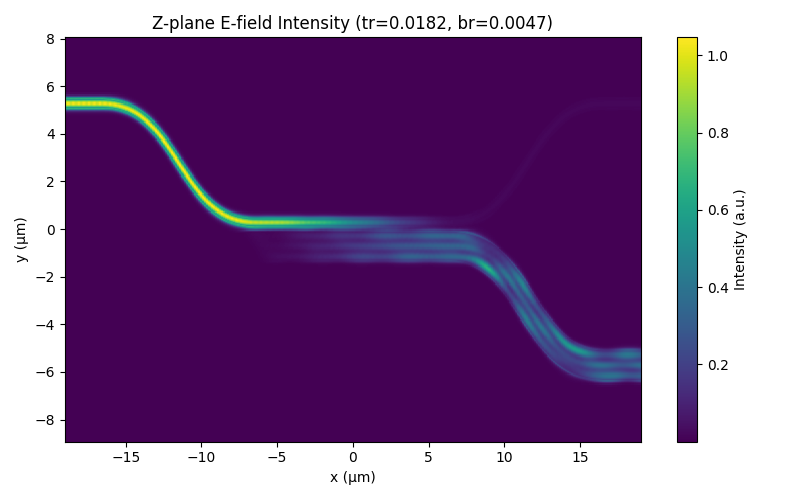
\includegraphics[width=0.8\textwidth]{task3/sim_1521_130625/z_plane_intensity.png}
  \caption{Power intensity distribution across the waveguide plane at the coupling length \(L=\hat{L}\approx\SI{13}{\um}\) for a fixed upper waveguide width of \(w_1=\SI{0.4}{\um}\), lower waveguide width of \(w_2=\SI{1.28}{\um}\), and separation gap of \(s=\SI{0.15}{\um}\) under input port TE\textsubscript{0} mode excitation at \SI{1550}{\nm}.}
  \label{fig:cross_mode_power_distribution}
\end{figure}



\section{Other contributions}


\section{Conclusion}


\printbibliography
\end{document}